\chapter{Käyttöjärjestelmäydin}

\label{kernel}

\section{Yleistä}

Perinteisesti käyttöjärjestelmäytimet, kernelit, jaetaan monoliittisiin- ja mikroytimiin. Monoliittinen ydin sisältää kaikki ytimen toiminnot yhdessä osoiteavaruudessa, yhdessä kokonaisuudessa. Se on usein tehokkaampi ja helpompi kehittää kuin mikroydin, joka koostuu monesta osasta. Mikroytimeen perustuva käyttöjärjestelmä koostuu \textit{moduuleista}, joita pelkistetty \textit{mikroydin} ohjaa. Moduulit ovat usein käyttäjätilassa, englanniksi userspace, ydintilan (kernel space) sijaan. Koostuessaan useasta moduulista kokonaisuus on usein vakaampi kuin monoliittinen ydin, mutta hitaampi ja monimutkaisempi. UNIX-johdannaiset, kuten Linux, ovat yleensä monoliittisia.

\section{Käynnistys}

X86-tietokoneen käynnistyessä prosessori alkaa suorittaa koodia BIOSin ROM -muistista. BIOSin avulla etsitään ja otetaan käyttöön muisti ja kaikki laitteet ja saatetaan laitteisto sellaiseen tilaan, että ohjaus voidaan siirtää käynnistyslataajalle (bootloader) ja edelleen käyttöjärjestelmän ytimelle. Käynnistyslataajan toimintaan ei tässä tutustuta tarkemmin.

\subsection{Ytimen ensimmäiset askeleet}
Käynnistyslataaja siirtää ohjauksen ytimelle, eli paremmin sanottuna siirtää prosessorin suorittamaan ytimen koodia ladattuaan sen massamuistista RAM-muistiin. RazOSin tapauksessa prosessori siirtyy suorittamaan koodia osoitteesta 0x100000, eli yhden megatavun kohdalta muistin alusta laskien. Aluksi luodaan ja alustetaan pino, stack, otetaan käyttöön liukulaskentaprosessori, FPU, ja lopuksi siirrytään suorittamaan C-koodia (listaus 1).

\par

Siirryttyään C-koodin puolelle, alkaa prosessori suorittaa kmain()-funktiota. Sen avulla alustetaan laitteistoa ja otetaan käyttöön virtuaalimuisti. Lopuksi siirrytään käyttäjätilaan.

\begin{listing}[H]
\begin{minted}[]{nasm}
start:
    mov esp, stack_end   ; Luo ja alusta pino eli stack
    push dword 0
    push dword 0
    mov ebp, esp

    ;; Anna pinon alku ja multiboot-tiedot kmain():lle
    push esp
    push ebx

    fninit               ; Ota kayttoon FPU
    mov eax, cr0
    or eax, 1 << 5
    mov cr0, eax

    cli                  ; Poista kaytosta keskeytykset
    call kmain           ; Siirry suorittamaan C-koodia
\end{minted}
\caption{Käynnistyskoodia; razos/kernel/src/boot.s}
\label{lst:boot}
\end{listing}

\section{Virtuaalimuisti ja muistinhallinta}
Käynnistyksen aikana prosessori on ns. \textit{real mode}-tilassa, eli se käyttäytyy kuin 8086. Muistia ei ole käytettävissä kuin yksi megatavu, koska muistiosoitteet ovat 20-bittisiä. Käynnistyslataaja, tässä tapauksessa GNU GRUB, asettaa prosessorin 80386:n mukaiseen \textit{protected mode}-tilaan, jossa mukaan tulee uusia ominaisuuksia, tärkeimpinä virtuaalimuisti ja sivutus (paging). Muistiosoitteet kasvavat 32-bittisiksi, jolloin suurin mahdollinen määrä muistia on neljä gigatavua. Tietokoneessa ei kuitenkaan aina ole neljää gigatavua muistia, mutta koko osoiteavaruus on silti käytetävissä \textit{virtuaalisuutensa} takia. Fyysinen muisti on jaettu paloiksi, sivuiksi, ja virtuaaliosoiteavaruuden käytössä olevat muistialueet on ``mapattu'' tiettyihin sivuihin. Virtuaalimuisti mahdollistaa sen, että prosessorin osoiteavaruuteen voidaan liittää muutakin kuin vain RAM-muistia eli käyttömuistia. Esimerkiksi laitteita, kuten näytönohjain, voidaan mapata joihinkin muistiosoitteisiin, jolloin niihin osoitteisiin kirjoitettaessa tieto kulkeekin näytönohjaimelle eikä RAM-muistiin.

\par

Toinen virtuaalimuistin etu on se, että osoiteavaruuden kirjanpito voidaan tehä prosessikohtaiseksi. Tällöin jokainen prosessi voi olla täysin tietämätön muista prosesseista, eikä sen tarvitse tietää mihin kohtaan \textit{fyysistä} musitia se on ladattu, koska jokaisen prosessin osoiteavaruus alkaa nollasta ja päättyy neljään gigatavuun, osoitteeseen 0xFFFFFFFF. Muistia on myös helpompi suojella, kun käyttöjärjestelmä saa tarkistettua jokaisen luku- ja kirjoitusoperaation ja voi määrittää sivukohtaisesti mitä prosessi saa muistilla tehdä. Fyysisen muistin sivusta käytetään usein englanninkielistä nimitystä \textit{frame}, ja virtuaalisen muistin sivusta nimitystä \textit{page}.

\begin{figure}[H]
\centering
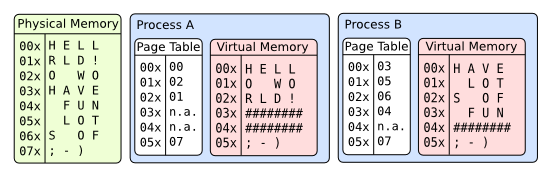
\includegraphics[width=\textwidth]{../figures/virtual_memory.png}
\caption{Virtuaalimuisti havainnollistettuna}
\label{fig:virtual_memory}
\end{figure}

\subsection{Virtuaalimuistin hallinta}

Muistinhallinnan perustehtäviä on varata ja vapauttaa muistia ohjelmien tarpeen mukaan, mahdollisimman tehokkaasti.

\subsubsection{Sivutus}

X86-arkkitehtuuri toteuttaa virtuaalimuistin sivutuksella, kun prosessori on protected mode -tilassa. Sivutuksen kirjanpito on kolmetasoinen:
\begin{figure}[H]
\centering
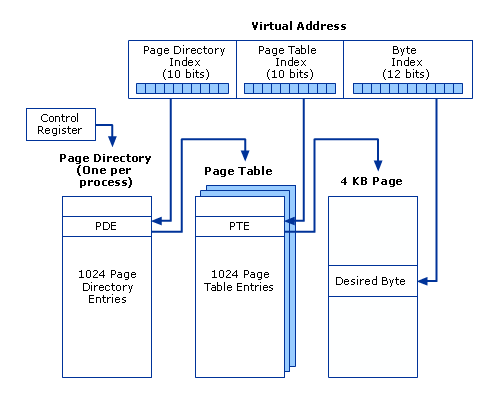
\includegraphics[width=\textwidth]{../figures/paging.png}
\caption{Sivutuksen kirjanpito}
\label{fig:paging}
\end{figure}

Prosessorin ohjausrekisteri CR3 sisältää kulloinkin käytössä olevan \textit{page directoryn} fyysisen muistiosoitteen. Page directory sisältää 1024 \textit{page directory entryä} (PDE), joiden \textit{flageilla} voi määrätä ominaisuuksia kutakin entryä vastaavaan \textit{page tableen}, joissa on jokaisessa puolestaan 1024 \textit{page table entryä} (PTE). PTE sisältää yhden neljän kilotavun sivun fyysisen osoitteen ja joitakin flageja, joiden avulla määritellään, onko esimerkiksi sivulle kirjoittaminen sallittua.

\par

Virtuaalinen muistiosoite on 32 bittiä pitkä. Sen 10 suurinta bittiä (bitit 31..21) ovat indeksi page directoryyn, eli kertovat mikä page table sisältää kyseisen sivun. Seuraavat kymmenen bittiä puolestaan ovat indeksi page tableen, eli kertovat mikä sivu on kyseessä. Loput 12 bittiä ovat halutun tavun etäisyys sivun alusta. RazOSissa page directory entryä kuvataan structilla pg\_dir\_entry\_t, ja page table entryä structilla page\_t.

\begin{listing}[H]
\begin{minted}[]{c}
struct page_t
{
	uint32_t present : 1;    /* Page present in memory */
	uint32_t rw : 1;         /* Page writable */
	uint32_t user : 1;       /* User-accessible */
	uint32_t wt_caching : 1; /* Write-through caching */
	uint32_t nocache : 1;    /* Caching disabled */
	uint32_t accessed : 1;   /* Has been accessed */
	uint32_t dirty : 1;      /* Has been written to */
	uint32_t zero : 1;       /* Always zero */
	uint32_t global : 1;     /* Global: do not flush in TLB flush */
	uint32_t avail : 3;      /* Bits not used by CPU */
	uint32_t frame : 20;     /* Physical address of the frame */
};

struct pg_dir_entry_t
{
	uint32_t present : 1;    /* Page present in memory */
	uint32_t rw : 1;         /* Page writable */
	uint32_t user : 1;       /* User-accessible */
	uint32_t wt_caching : 1; /* Write-through caching */
	uint32_t nocache : 1;    /* Caching disabled */
	uint32_t accessed : 1;   /* Has been accessed */
	uint32_t zero : 1;       /* Always zero */
	uint32_t size : 1;       /* 0 = 4K, 1 = 4M pages */
	uint32_t global : 1;     /* Global: do not flush in TLB flush */
	uint32_t avail : 3;      /* Bits not used by CPU */
	uint32_t table : 20;     /* Physical address of the page table */
};
\end{minted}
\caption{Sivutuksen tietorakenteita RazOSissa}
\label{lst:paging_structs}
\end{listing}

\par

Kun tarvitaan lisää muistia, aloitetaan etsimällä vapaa fyysinen sivu. RazOSissa sen hoitaa \texttt{frame\_alloc()}, joka palauttaa sivun fyysisen osoitteen. Tämän jälkeen sivu mapataan haluttuun virtuaaliosoitteeseen funktion \texttt{page\_map()} avulla. Se asettaa myös halutut flagit, esimerkiksi onko sivu vain ytimen käytössä vai saako käyttäjätason ohjelmatkin käyttää sitä. Tämän jälkeen tehdään ``TLB Flush'', eli tyhjennetään prosessorin välimuistista kyseistä virtuaaliosoitetta vastaava fyysinen osoite, jotta prosessori laskee uuden, jolloin muistioperaatiot tapahtuvat oikeassa, uudessa kohdassa fyysistä muistia. Muistin vapauttaminen toimii samalla tavalla, ensin poistetaan mappaus kyseisestä virtuaaliosoitteesta, merkitään sivu poissaolevaksi ja lopuksi merkitään fyysinen sivu vapaaksi funktiolla \texttt{frame\_free()}.

\subsubsection{Muistin varaaminen}

Kun muistia halutaan käyttää, täytyy sitä varata. Muistia käytetään pääosin kolmella tavalla: on pino (stack), dynaaminen muistialue (heap) sekä ohjelmakoodille varattu, suoritettava alue. Yksittäiset muuttujat tallennetaan yleensä pinoon, ja esimerkiksi funktiota kutsuttaessa sen parametrit ja paluuosoite tallennetaan pinoon. Heappiä käytetään dynaamiseen varaukseen ja vapautukseen esimerkiksi suurten listojen kanssa. Pino on kooltaan hyvin pieni, kun heap puolestaan on todella suuri: RazOSissa pinon koko on 64 kilotavua, heapille on varattu virtuaaliosoitteita yli kolmen gigatavun edestä.

\par

Muistin varaaminen heapiltä tapahtuu C-standardin mukaan \texttt{malloc()}-perheen funktioilla. Malloc tarvitsee tosin heap-alueen toimiakseen, ja sen käsittelyyn, laajentamiseen ja pienentämiseen, on perinteisesti kaksi funktiota; \texttt{brk()} ja \texttt{sbrk()}, jotka POSIX ennen määritteli. Funktiot \texttt{brk()} ja \texttt{sbrk()} käyttävät funktiota \texttt{page\_map()} sivujen varaamiseen ja vapauttamiseen. Nykyään standardiin kuuluu niiden sijaan \texttt{mmap()}, mutta sen tarkastelu sivuutetaan. Malloc -implementaatioita on useita, joista ehkä tunnetuin on Doug Lean malloc, dlmalloc. Dlmalloc on melko joustava, ja siksi sitä käytetään paljon \parencite{dlmalloc}. Muitakin implementaatioita on tehty, joissakin on tarkoituksena säästää muistia ja toisissa prosessoriaikaa.

\par

RazOSin malloc, rmalloc, lainaa joitain dlmallocin ajatuksia, ja on hyvin yksinkertainen. Rmallocista on kaksi eri versiota; toinen ytimen käyttöön ja toinen käyttäjämaailman prosessien käyttöön. Käyttäjämaailman toimintaa tarkastellaan myöhemmin. Funktioiden ero on siinä, miten varattu muisti sijoitetaan osoiteavaruuteen: ytimelle on monissa tapauksissa tärkeää, että osoitteet ovat esimerkiksi jaollisia yhden sivun koolla, neljällä kilotavulla. Käyttäjämaailmassa ei tällaista rajoitusta ole, joten käyttäjämaailman rmalloc on hieman yksinkertaisempi.

\begin{figure}[H]
\centering
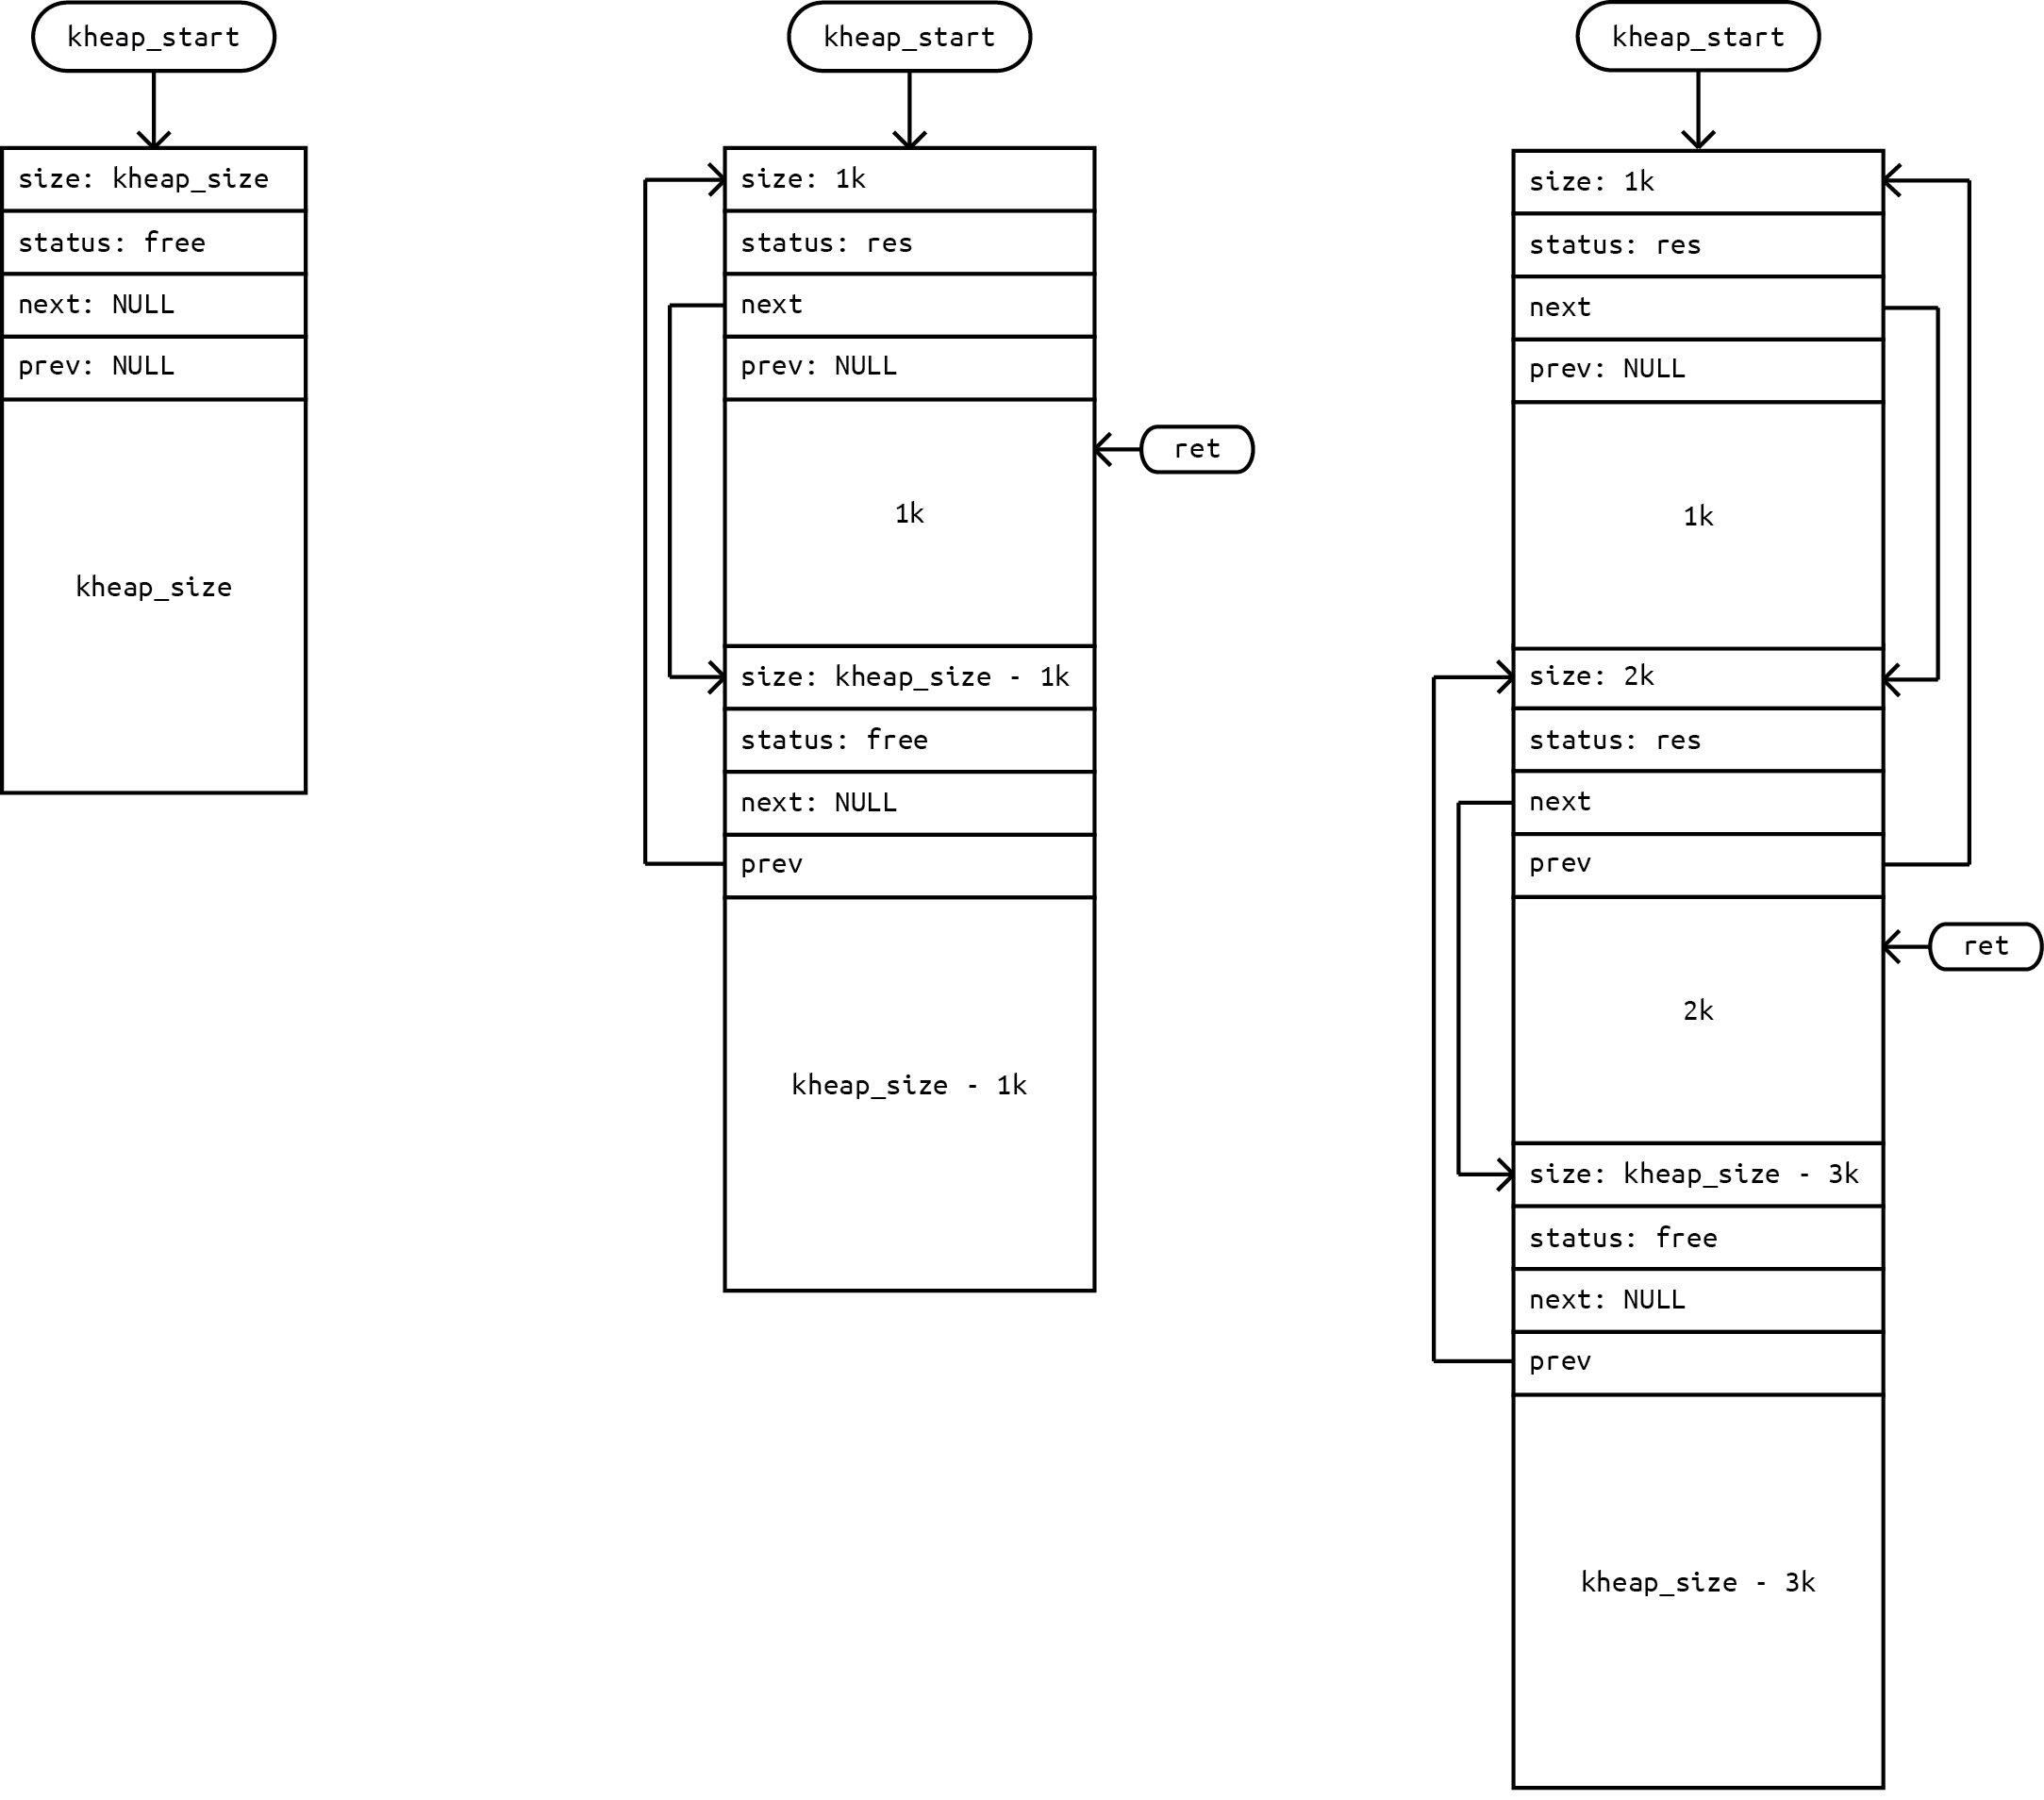
\includegraphics[width=\textwidth]{../figures/rmalloc.png}
\caption{Graafi rmallocin toiminnasta. Alkutilanne, yksi yhden kilotavun varaus ja viimeisessä toinen, kahden kilotavun varaus.}
\label{fig:rmalloc}
\end{figure}

\subsubsection{Muistin vapauttaminen}
Kun halutaan vapauttaa muistia heapiltä, käytetään perinteisesti funktiota \texttt{free()}. Se merkitsee mallocilla varatun muistin vapaaksi, yhdistää läheiset vapaat muistialueet (coalescing) ja mikäli mahdollista, pienetää heap-aluetta \texttt{sbrk()}:n avulla.

\begin{figure}[H]
\centering
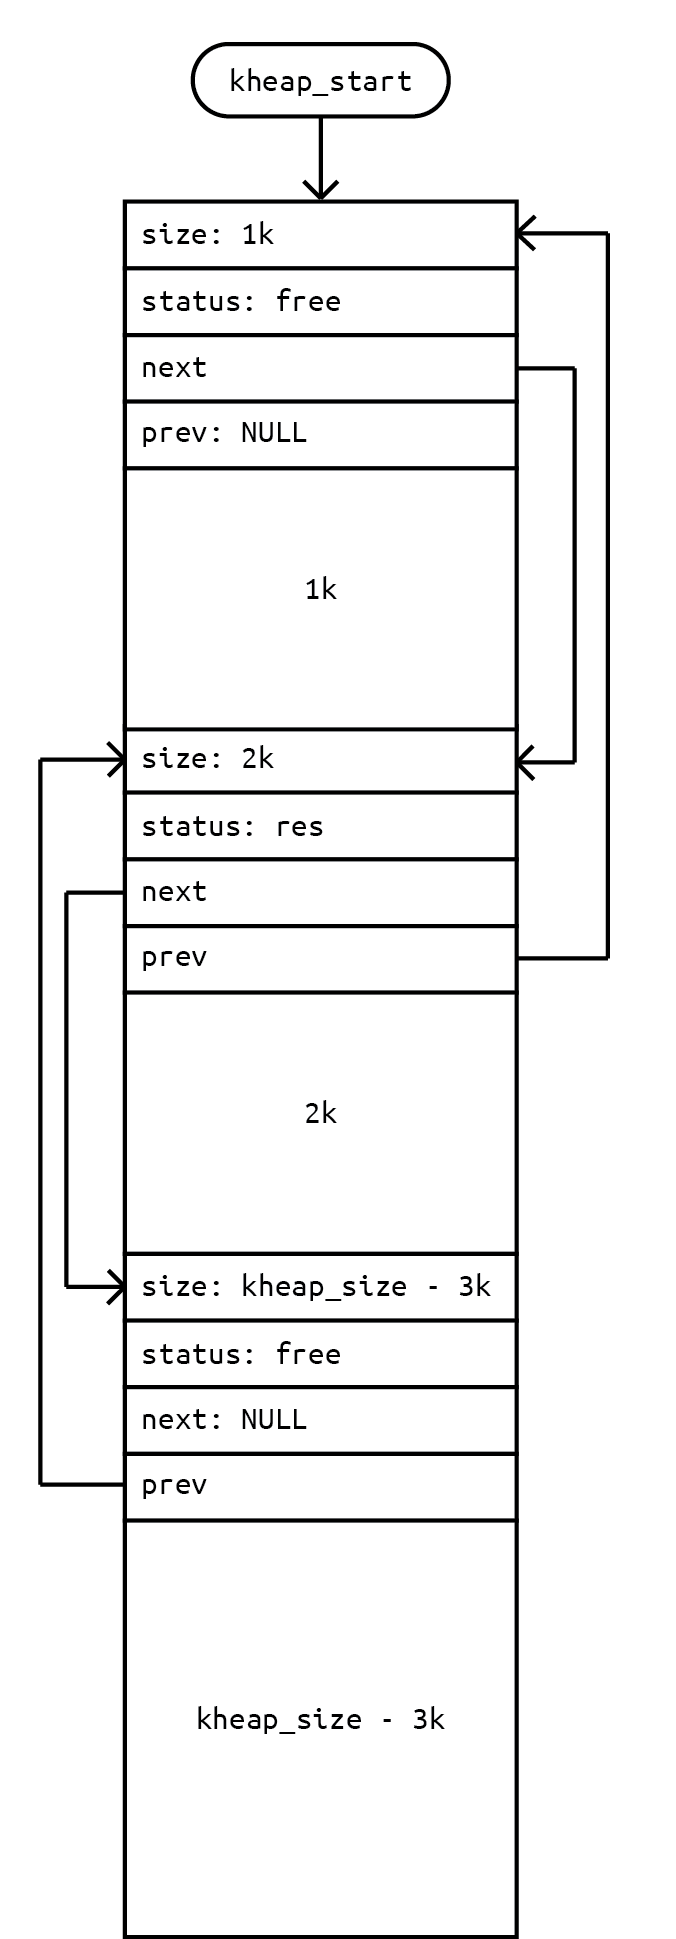
\includegraphics[]{../figures/rfree.png}
\caption{Kuvan \ref{fig:rmalloc} viimeisen tapauksen mukaisesta heapistä on vapautettu ensimmäinen, yhden kilotavun varaus.}
\label{fig:rfree}
\end{figure}

\section{Keskeytykset}

Keskeytys (interrupt) on joko laitteiston tai ohjelman aikaansaama signaali, joka keskeyttää prosessorin toiminnan. Keskeytyksen tullessa suoritin tallentaa tilansa pinoon, ja siirtyy suorittamaan keskeytyskäsittelijää (interrupt handler). Kun käsittelijän suoritus on saatu päätökseen, palauttaa prosessori tilansa pinosta ja jatkaa siitä, mihin jäi keskeytyksen tullessa. Keskeytyksiä käytetään yleensä siihen, että tietokone saa tiedon erinäisitä tapahtumista, kuten näppäimistön napin painalluksista tai ajastimen (PIT, programmable interrupt timer) laukeamisesta. Tällöin prosessorin ei tarvitse koko ajan tarkistaa, onko jotain tapahtunut, jolloin prosessoriaikaa säästyy.

\par

X86-arkkitehtuurilla keskeytyskäsittelijöiden sijainti on tallennettu IDT-taulukkoon (Interrupt Descriptor Table). Jokainen keskeytys on numeroitu, ja IDT:stä löytyy jokaista numeroa vastaavan käsittelijän osoite, johon prosessori hyppää keskeytyksen tullessa.

\subsection{Poikkeukset}

Poikkeukset (exception) ovat keskeytyksiä, joita prosessori itse aiheuttaa. Tyypillisiä poikkeus ovat nollalla jako ja sivutusvirhe (page fault). Niiden tullessa, on prosessori yrittänyt suorittaa jotain käskyä siinä onnistumatta.

\subsubsection {Sivutusvirhe}

Sivutusvirhe tulee, kun yritetään käyttää muistia, jota ei ole mapattu tai jota ei saa käyttää. Sivutusvirheen virhekoodi kertoo, mikä meni pieleen; eikö muistia oltu mapattu, eikö muistiin kirjoittaminen ollut sallittua tai eikö käyttäjätason ohjelma saanut siihen koskea. Virheen käsittelijä voi olla hyvinkin monimutkainen, sillä se voi yrittää korjata tilannetta. Esimerkiksi Linux tukee niin sanottua \textit{demand pagingiä}, jossa virtuaaliosoitetta ei mapata fyysiseen sivuun ennen ensimmäistä käyttöyritystä. Tällöin säästetään fyysistä muistia muiden prosessien käyttöön.

\par

Yksinkertaisimmillaan käsittelijä vain ilmoittaa ongelmasta ja lopettaa ongelman aiheuttaneen ohjelman suorituksen. Yleensä ongelma tosin pyritään korjaamaan, mutta se ei aina ole mahdollista. Silloin UNIX-variantit lähettävät \texttt{SIGSEGV} -signaalin, jolla prosessi lopetetaan. RazOS ei vielä tue signaaleja, joten RazOSin sivutusvirhekäsittelijä vain lopettaa suorituksen.

\subsection{Laitteistokeskeytykset}

Laitteistokeskeytykset (Interrupt request, IRQ) aiheutuvat laitteiston toiminnasta. Esimerkiksi näppäimistön nappia painettaessa lähtee prosessorille tieto keskeytyksestä numero 33, jolloin prosessori etsii IDT:stä oikean käsittelijän ja hyppää siihen. Aluksi tallennetaan prosessorin tila, kerrotaan näppäimistölle, että keskeytys on huomattu ja jatketaan keskeytyksen käsittelyä.

\begin{listing}[H]
\begin{minted}[]{nasm}
isr_33:
    pusha           ; Prosessorin tilan tallennus pinoon

    ;; Ilmoitetaan nappaimistolle keskeytyksen huomaamisesta
    push ax
    mov al, 0x20
    out 0xa0, al
    out 0x20, al
    pop ax

    call kb_handler ; Hypataan C-koodin puolelle
    popa            ; Palautetaan prosessorin tila
    iret            ; Jatketaan suoritusta siita, mihin jaatiin
\end{minted}
\caption{Näppäimistökeskeytyksen käsittely; razos/kernel/src/drivers/isr.s}
\label{lst:kb_isr}
\end{listing}

\section{Moniajo}

Moderni käyttöjärjestelmä kykenee moniajoon, eli sillä voi käyttää useampaa ohjelmaa samaan aikaan. Myös UNIX ja sen variantit kykenevät siihen, myös RazOS. Moniytiminen prosessori kykenee suorittamaan useaa prosessia samaan aikaan, mutta tässä tarkastellaan vain yksiytimisiä prosessoreita, joissa moniajo toteutetaan jakamalla prosessoriaika usean prosessin (säikeen, thread of execution) välillä. Oiva työkalu siihen on ajastimen aiheuttamat keskeytykset; ajastimen keskeytyskäsittelijä vaihtaa suoritettavan prosessin aina ajastimen lauetessa.

\subsection{Moniajo UNIX-varianteissa}

\subsubsection{fork-exec}

UNIX ja sen variantit, mukaan lukien RazOS, hoitavat moniajon ja uuden prosessin aloituksen niin sanotulla \textit{fork-exec} -menetelmällä. Siinä käytetään funktiota \texttt{fork()} kopioimaan jonkin prosessin (vanhempi, parent) osoiteavaruus, jolloin syntyy toinen, samaa koodia suorittava prosessi (lapsi, child). Lapsi jatkaa suoritusta samasta kohdasta vanhempansa kanssa, mutta sillä on oma kopionsa muistista käytössä, ja se siis työskentelee omassa osoiteavaruudessaan, jolloin sillä on oma \textit{page directory}. Tämän jälkeen voidaan kutsua jotain \texttt{exec}-perheen funktiota, RazOSissa \texttt{execve()} tai \texttt{execv()}, jolla vaihdetaan suoritettava koodi (process image), eli siirrytään suorittamaan eri ohjelmaa. Prosesseista käytetään UNIX-termiä \textit{task}. Kun lapsi on suoritettu loppuun, kutsutaan C-kirjaston funktiota \texttt{exit()}, joka siirtää suorituksen ytimelle. Ydin vapauttaa lapsen varaaman muistin ja ilmottaa sen vanhemmalle lapsen ``kuolleen'' ja kertoo sen palautusarvon. Tämän jälkeen kaikki jäänteet lapsesta siivotaan muistista, ja palataan suorittamaan muita prosesseja.

\par

RazOSissa jokaista prosessia kuvaa \texttt{struct task\_t}, joka sisältää kaiken oleellisen tiedon prosessista:

\begin{listing}[H]
\begin{minted}[]{c}
struct task_t
{
	uint8_t fpu_state[512];      /* Liukulukuprosessorin tila */
	uint32_t esp;                /* Pinon alku */
	uint32_t eip;                /* Suoritettavan kaskyn osoite */
	struct page_dir_t* page_dir;

	struct registers_t* syscall_regs; /* Prosessorin rekisterit */

	pid_t pid;                   /* Prosessin numero */
	pid_t ppid;                  /* Vanhemman numero */

	uint32_t state;
	uint32_t exit_status;        /* Palautusarvo */

	uint32_t children;           /* Lapsien maara */

	struct task_t* wait_queue;   /* ``Kuolleiden'' lasten lista */

	void* uheap_begin;           /* Kayttajapuolen heap-alueen alku */
	void* uheap_end;

	struct fildes_t files[OPEN_MAX]; /* Kaytossa olevat tiedostot */
	int* errno_loc;              /* errno-virhekoodin osoite */
};
\end{minted}
\caption{task\_t; razos/kernel/src/mm/task.h}
\label{lst:task_t}
\end{listing}

\par

Funktion \texttt{fork()} implementaatioon voi tutustua tiedostojen \texttt{razos/kernel/src/mm/task.c} ja \texttt{razos/kernel/src/mm/task.s} avulla.

\subsubsection{Ohjelman lataus}

Tietokoneohjelmia tehdään monessa muodossa. UNIX-maailmassa niistä yleisin on ELF (Executable and Linkable Format). ELF-tiedosto pitää sisällään ohjelmakoodin, etukäteen alustetut muuttujat (kuten merkkijonot) ja ohjeet käyttöjärjestelmälle siitä, miten tiedosto kuuluu ladata (virtuaali-) muistiin. Lataaja avaa tiedoston ja kopioi sen sisällön ohjeiden mukaan oikeisiin kohtiin osoiteavaruutta. Tämän jälkeen suoritus siirtyy uuden ohjelman alkuun.

\par

Ohjelman lataukseen käytetään jotain \texttt{exec()}-funktioista. Ne antavat ohjelmalle lisäksi argumentteja ja ympäristömuuttujia (environment variable). Funktio vapauttaa käyttäjän muistialueet, sulkee avoimet tiedostot ja vaihtaa ohjelmakoodin. RazOSissa \texttt{exec()}-funktioperheen kaikki funktiot perustuvat funktioon \texttt{execve()}. Sen lähdekoodi löytyy kansiosta \texttt{razos/kernel/src/loader/}.

\subsubsection{Prosessin vaihto}

Ajastimen lauetessa kutsutaan vuorontajaa (scheduler), joka valitsee seuraavan suoritettavan prosessin. Aluksi vuorontaja tallentaa vanhan prosessin tilan, RazOSissa \texttt{task\_t}:hen, jotta sen suoritukseen voidaan myöhemmin palata ongelmitta. Sen jälkeen valitaan uusi prosessi funktiolla \texttt{sched\_next()}, vaihdetaan osoiteavaruus eli kirjoitetaan \texttt{CR3}-ohjausrekisteriin uuden prosessin page directoryn osoite ja lopuksi palautetaan uuden prosessin tila \texttt{task\_t}:stä. Tämän jälkeen vuorontajan suoritus loppuu ja hypätään \texttt{task\_t}:stä otettuun suoritusosoitteeseen (rekisteri EIP, [Extended] Instruction Pointer), josta palataan usein käyttäjämaailmaan ja siellä jatketaan prosessin suoritusta seuraavaan ajastimen laukeamiseen asti.

\begin{listing}[H]
\begin{minted}[]{nasm}
sched_switch:
    ;; Tallenna vanhan prosessin tila
    pusha
    mov eax, [cur_task]
    fxsave task_fpu_state(eax)
    mov task_esp(eax), esp
    mov task_eip(eax), dword .return ; Osoite, josta suoritus jatkuu

    ;; Valitse uusi prosessi
    call sched_next
    mov [cur_task], eax

    ;; Hae page directoryn fyysinen osoite
    push dword task_page_dir(eax)
    call get_page_dir_phys
    add esp, 4

    ;; Lataa se CR3:een
    mov cr3, eax

    mov eax, [cur_task]

    ;; Palauta prosessin tila
    fxrstor task_fpu_state(eax)
    mov esp, task_esp(eax)
    jmp task_eip(eax)

.return:
    popa
    ret
\end{minted}
\caption{Vuorontajan assemblyllä kirjoitettu osa; razos/kernel/src/mm/task.s}
\label{lst:sched_switch}
\end{listing}

\par

Vuoronnusalgoritmeja on useita. Yleensä prosesseille voidaan määrittää prioriteetti, jonka mukaan määrätään mikä prosessi saa eniten suoritusaikaa. Yksinkertaisissa algoritmeissa ei priorisointia ole. Esimerkiksi RazOS käyttää nk. kiertovuorottelumenetelmää (round robin scheduling), jossa jokainen prosessi saa käyttää aikaa korkeintaan jonkin tietyn aikaviipaleen (time slice) verran. Tämän jälkeen prosessia vaihdetaan ja ajossa ollut prosessi laitetaan jonon viimeiseksi. Menetelmä on \textit{irrottava}, koska ydin voi määrätä milloin prosessin aikaviipale loppuu ja on vaihdettava prosessia. Irrottavan vuoronnuksen vastakohta on ei-irrottava vuoronnus, jossa prosessilta ei voida viedä vuoroa pois, vaan se luovuttaa sen itse. Sekin on usein mahdollista irrottavaa vuoronnusta käyttävissä järjestelmissä. Esimerkiksi RazOSissa prosessi antaa suoritusvuoronsa pois, jos se joutuu odottamaan esimerkiksi lukuoperaation valmistumista. Siihen käytetään funktiota \texttt{sched\_yield()}.

\section{Tiedostojen hallinta}

Yksi käyttöjärjestelmän tärkeistä osista on tiedostojen hallitseminen. Se on laaja kokonaisuus, jossa noustaan abstraktiotasolta toiselle, kunnes C-kirjaston yleiset metodit (tiedostossa \texttt{stdio.h}) ovat käytettävissä. POSIX tuo omia keinojaan, jotka ovat abstraktioltaan paljon alempana C-kirjastoa. Abstraktion tarkoituksena on, että ohjelmoija voi samalla tavalla käyttää mitä tahansa tiedostoksi ajateltavaa kokonaisuutta: kiintolevyllä olevaa tiedostoa, sarjaporttia tai vaikkapa USB-väylää. Abstraktiota kutsutaan virtuaalitiedostojärjestelmäksi (Virtual File System, VFS). RazOSissa VFS kuvaa tiedostoja ja niihin verrattavia kokonaisuuksia structeilla \texttt{vfs\_node\_t} ja \texttt{stat} ja käsittelee avoimia tiedostoja structin \texttt{fildes\_t} avulla.

\begin{listing}[H]
\begin{minted}[]{c}
struct vfs_node_t
{
	char name[64];      /* Tiedoston nimi */
	struct stat status;

    /* Kyseisen tiedostojarjestelman kasittelyfunktiot,
     * kuuluvat laitteen/tiedostojarjestelman ajuriin */
	read_t read;
	write_t write;
	open_t open;
	creat_t creat;
	close_t close;
	lseek_t lseek;

    /* VFS on linkitetty lista, osoitin seuraavaan alkioon */
	struct vfs_node_t* next;
};

struct fildes_t
{
	struct vfs_node_t* vfs_node;
	off_t at;       /* Kertoo missa kohdassa tiedostoa ollaan */
	uint32_t oflag; /* Tiedoston avausflagit */
};
\end{minted}
\caption{vfs\_node\_t ja fildes\_t; razos/kernel/src/fs/vfs.h}
\label{lst:sched_switch}
\end{listing}

Structi stat löytyy tiedostosta \texttt{razos/razos\_kernel\_headers/sys/stat.h}. Se pitää sisällään tiedostoa koskevaa tietoa, kuten millä laitteella se sijaitsee (vai onko se laite itsessään), mitä sille saa tehdä, ja koska sitä on viimeksi muokattu.

\par

Kun jotain tiedostoa halutaan käyttää, tulee se ensin avata funktiolla \texttt{open()}. Se palauttaa numeron, file descriptorin (fd), joka viittaa johonkin prosessin \texttt{task\_t}:ssä olevista \texttt{fildes\_t} -structeista. Se pitää sisällään avausflagit ja pitää kirjaa missä kohdassa tiedostoa ollaan. Siinä on myös osoitin tiedostoa vastaavaan \texttt{vfs\_node\_t} -structiin, jonka kautta löydetään sopivat funktiot tiedoston käyttöön. Funktioista löytyy tietoa standardeista \parencite{POSIX} ja \parencite{ISOC99} ja niiden implementaatiot löytyvät kansiosta \texttt{razos/kernel/src/fs/}.

\par

Tiedostoja on monenlaisia. Tavallisten tiedostojen ja laitteiden lisäksi UNIX käsittelee putkia (pipe), joiden kautta prosessit voivat lähettää toisilleen tietoa. Putki on sisäisesti jono (FIFO, first-in, first-out), jonka päät ovat eri prosesseissa. Lisäksi on näytölle tulostamista varten \texttt{stdout} ja \texttt{stderr} ja näppäimistöltä lukemista varten \texttt{stdin}. Niitä voidaan korvata putkilla, jolloin yksi prosessi voi lähettää tavallisesti näytölle tulostettavan tekstin toiselle prosessille, joka käsittelee sen kuin se olisi tullut näppäimistöltä.

\section{Järjestelmäkutsut}

Järjestelmäkutsut eli system callit (syscall) mahdollistavat käyttäjätason ohjelmien pääsyn ytimen resursseihin turvallisesti. X86-alustalla järjestelmäkutsuja voidaan toteuttaa usealla tavalla, joista yleisimmät ovat keskeytysten käyttö tai \texttt{sysenter} ja \texttt{sysexit} -käskyjen käyttö. Keskeytyksien käyttö on usein hitaampaa, ja RazOS käyttääkin jälkimmäistä keinoa. Suorittaessaan \texttt{sysenter}-komennon, siirtyy prosessori lupatasoista (current privilege level, CPL) suurimmalle, tasolle nolla. Käyttäjämaailman koodia ajetaan tasolla kolme. Tasojen erot ovat siinä, että 0-tasolla on käytettävissä joitain käskyjä, jotka saattavat saada vahinkoa aikaan, jos esimerkiksi haittaohjelma pystyisi niitä suorittamaan. Toinen ero on se, että sivutuksen avulla voidaan määritellä, mitä muistia 3-tason koodi saa käyttää. Suoritustason muutoksen lisäksi prosessori siirtyy suorittamaan koodia, jonka osoite on tallennettu MSR-rekisteriin. Sieltä suoritus etenee haluttuun järjestelmäkutsuun, ja lopuksi palataan käyttäjämaailmaan, tasolle 3, käskyllä \texttt{sysexit}.  Käskyjen toimintaan ja lupatasoihin voi tutustua tarkemmin Intelin manuaalin avulla \parencite{INTEL_MAN}.

\par

Järjestelmäkutsut on numeroitu, ja niiden numerot löytyvät RazOSissa tiedostosta \texttt{razos/razos\_kernel\_headers/api/razos.h}. Kun käyttäjätason koodissa halutaan käyttää jotain järjestelmäkutsua, käytetään siihen tiedostosta \texttt{razos/rlibc/arch/i386/crt0.s} löytyviä \texttt{\_\_syscall} -funktioita. Niille annetaan argumenteiksi järjestelmäkutsun numero ja mahdolliset muut parametrit, maksimissaan kolme.

\begin{listing}[H]
\begin{minted}[]{nasm}
    ;; Parametrit ja syscall-numero System V ABI:n mukaisesti pinossa
    ;; razos.h:ssa uint32_t __syscall3(num, arg1, arg2, arg3)
__syscall3:
    ;; Tallennetaan callee-save rekisterit (System V ABI)
    push ebx
    push edi
    push esi

    ;; Parametrit ja syscall-numero pinosta rekistereihin
    mov esi, [esp+12+16]
    mov edi, [esp+12+12]
    mov ebx, [esp+12+8]
    mov eax, [esp+12+4]

    ;; sysexit vaatii kayttajamaailman pinon (esp)
    ;; ja osoitteen, josta suoritusta jatketaan kutsun
    ;; jalkeen rekistereihin ecx ja edx
    push ecx
    push edx
    mov ecx, esp
    mov edx, .ret
    sysenter

    ;; Kutsusta palataan tahan sysexitin avulla
.ret:
    ;; Palautetaan rekisterien arvot pinosta
    pop edx
    pop ecx
    pop esi
    pop edi
    pop ebx

    ;; Palataan sinne, mista syscallia kutsuttiin
    ret
\end{minted}
\caption{\texttt{\_\_syscall} -funktioista yksi, kolme argumenttia ottava}
\label{lst:syscall3}
\end{listing}

Ylläolevasta koodista hypätään \texttt{sysenter}illä ytimeen, funktioon \texttt{syscall\_entry}, tiedostossa \texttt{razos/kernel/src/syscall/syscall.s}. Siellä alustetaan kernelin pino ja kutsutaan C-koodilla kirjoitettu jatkokäsittelijä, \texttt{syscall\_dispatch()}. Se etsii \texttt{syscall\_table} -taulukosta järjestelmäkutsun numeroa vastaavan funktion, ja suorittaa sen. Lopuksi siivotaan pino ja suoritetaan \texttt{sysexit} -komento, jonka myötä palataan käyttäjämaailmaan.

\par

Järjestelmäkutsujen avulla voidaan kirjoittaa C-kirjaston ne osat, jotka tarvitsevat jotain kernelin resursseja, kuten tiedostoja. Ilman niitä olisi kirjaston teko hyvin vaikeaa, ja ohjelmien pitäisi olla osa ydintä. Se veisi mennessään huomattavan paljon joustavuutta ja toisi mukanaan suuria tietoturvaongelmia, koska kaikki koodi voisi käyttää mitä vain ytimen osaa hyväkseen, ja kaikki koodi suoritettaisiin lupatasolla nolla.